\section{Adjusted mutual information analysis}
	This section summarizes the adjusted mutual information project for a dataset generated using an arbitrary transfer matrix for a 19 fibre Photonic Lantern.
	
	
	\subsection{Purpose}
	
		The purpose is to determine wether if the problem in the section above is from the RSoft transfer matrix or the clustering algorithm information loss.\\
		
		To do this we generate a transfer matrix with a condition number of 1 and again check the AMI between the different spaces for a dataset of 10000 points created with 9 Zernike modes.\\
		
		When the datasets are created we use K-Means clustering to group points and measure AMI\\
		
		
	\subsection{The data}
		There are 6 different types of datasets:
		\begin{itemize}
			\item Zernike coefficients
			\item PSF intensities
			\item PSF complex fields
			\item LP coefficients
			\item Photonic Lantern Output fluxes
			\item Photonic Lanter Output complex amplitudes
		\end{itemize}
		
		The paths to the datasets used to check how the AMI evolves with the number on points of the dataset can be found in \href{https://github.com/Dacarpe03/PLImageReconstruction/blob/main/Utils/ami_analysis_constants.py}{ami\_analysis\_constants.py}.
		
	
	\subsection{Results}
		\begin{figure*}[ht!]
			\centering
			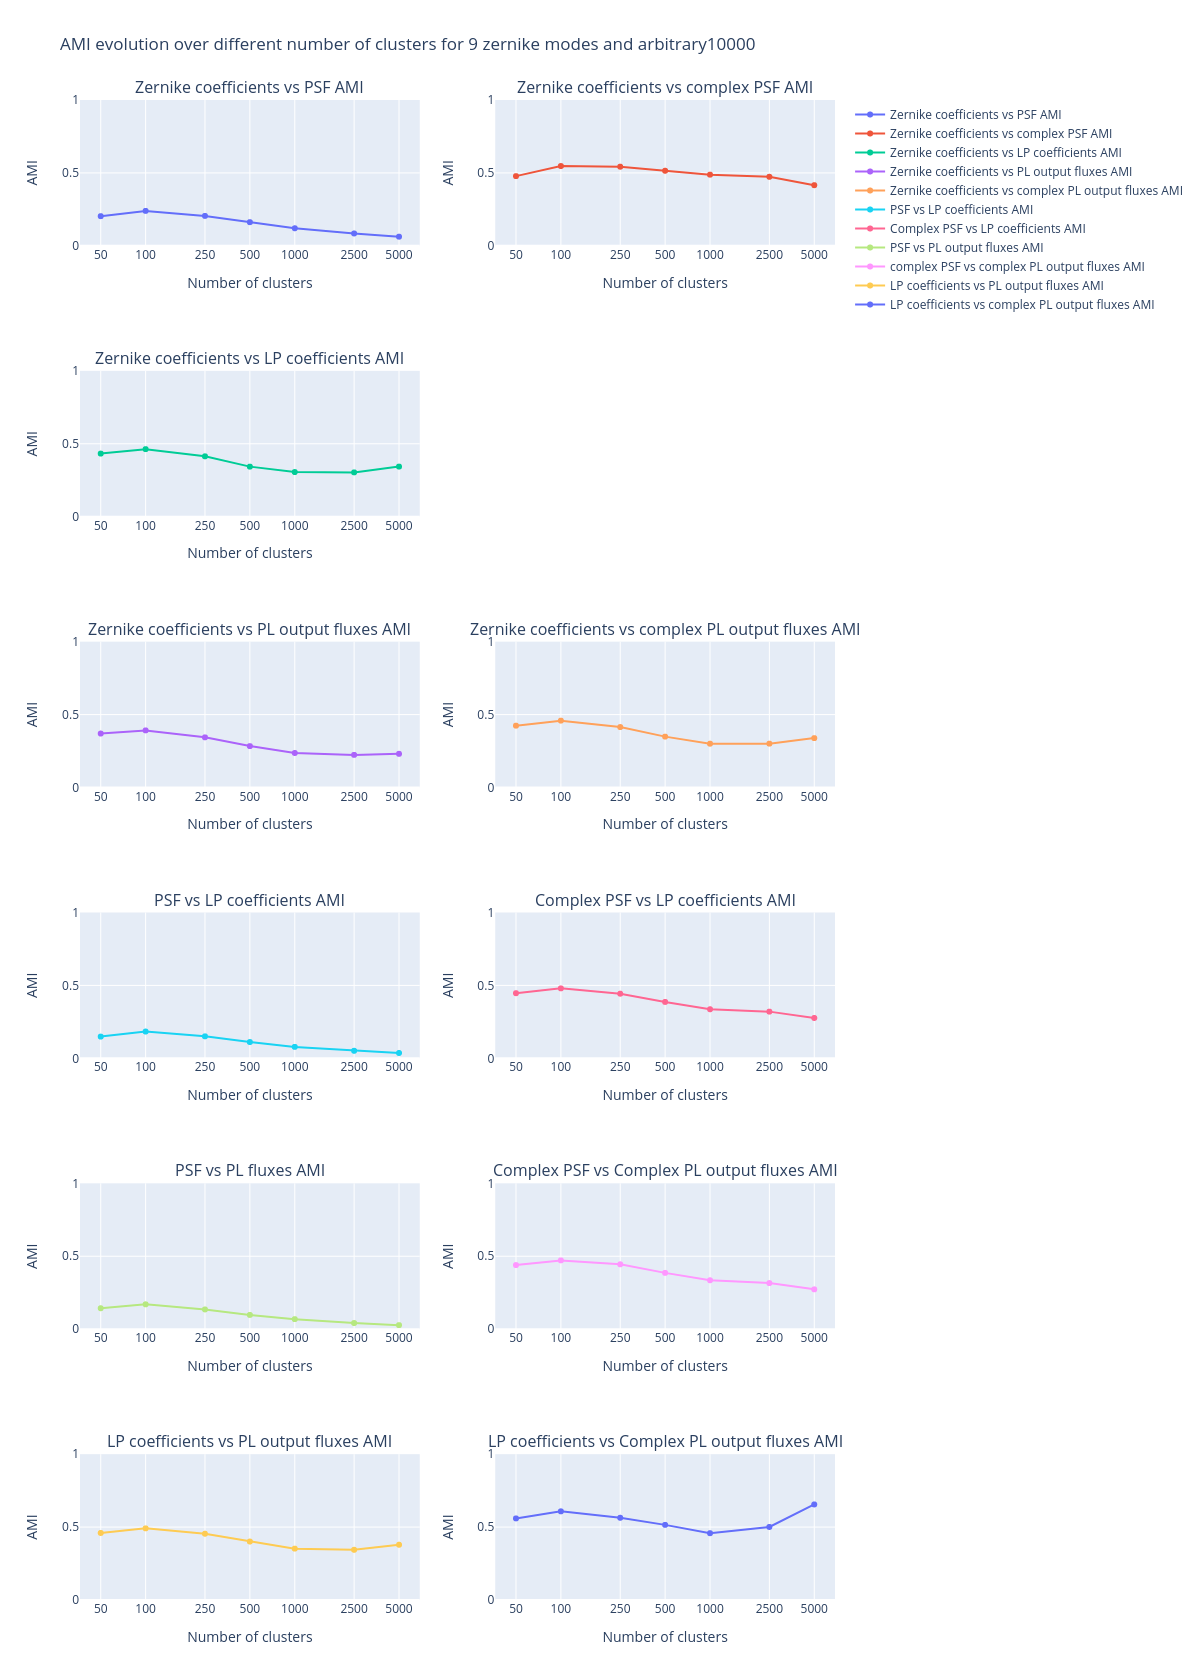
\includegraphics[width=0.9\textwidth]{ld-amievolutionoverarbitrary10000.png}
		\end{figure*}
		\FloatBarrier
		
		The AMI between LP coefficients and PL complex amplitudes is still not high after using an arbitrary transfer matrix. The problem seems to be in the clustering process where information is loss, or maybe there is something that we are still missing in the model.\\
		
	
	\subsection{Code}
	
	Code for AMI analysis over dataset size:
	\begin{itemize}
		\item The data generation for the AMI analysis over dataset size can be found in \href{https://github.com/Dacarpe03/PLImageReconstruction/blob/main/PSFReconstruction/Scripts/TrueLastLastDanceDatasetZernikePSFGeneration.py}{TrueLastLastDanceDatasetZernikePSFGeneration.py}
		\item The data processing for the AMI analysis over dataset size can be found in \href{https://github.com/Dacarpe03/PLImageReconstruction/blob/main/PSFReconstruction/Scripts/TrueLastLastDancedatasetProcessing.py}{TrueLastLastDancedatasetProcessing.py}
		\item The dimensionality reduction of the data for the AMI analysis over dataset size can be found in \href{https://github.com/Dacarpe03/PLImageReconstruction/blob/main/PSFReconstruction/Scripts/TrueLastLastDanceDatasetDimensionalityReduction.py}{TrueLastLastDanceDatasetDimensionalityReduction.py}
		\item The clustering of the data for the AMI analysis over dataset size can be found in \href{https://github.com/Dacarpe03/PLImageReconstruction/blob/main/PSFReconstruction/Scripts/TrueLastLastDanceDatasetClustering.py}{TrueLastLastDanceDatasetClustering.py}
		\item The plots and AMI analysis over number of Zernike Modes can be found in \href{https://github.com/Dacarpe03/PLImageReconstruction/blob/main/PSFReconstruction/DataNotebooks/LastDanceAMIAnalysisOverNClusters.ipynb}{LastDanceAMIAnalysisOverNClusters.ipynb}
	\end{itemize}
	